\subsection{Rancangan Detail Komponen Reporting}
\label{subsection:detail-reporting}

Komponen \textit{reporting} bertanggung jawab untuk menghasilkan laporan berdasarkan data yang telah dikumpulkan oleh komponen \textit{data collector}. Komponen ini akan memproses data dan menghasilkan visualisasi yang dapat digunakan untuk analisis lebih lanjut.

Ilustrasi struktur komponen \textit{reporting} dapat dilihat pada gambar \ref{fig:reporting-structure}.

% _TODO: Change image
\begin{figure}[ht]
    \centering
    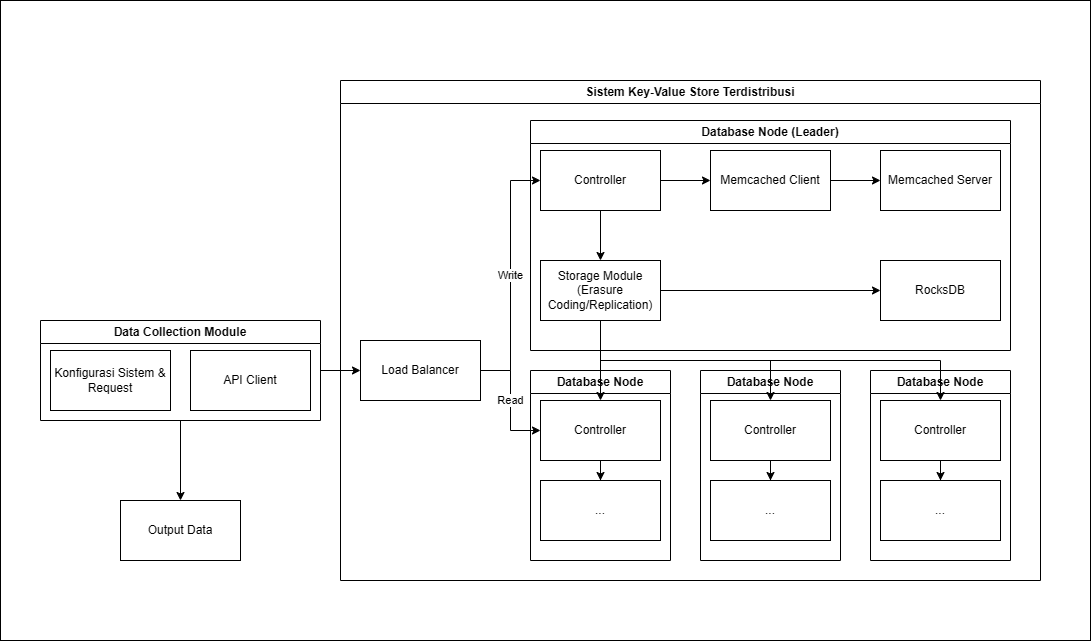
\includegraphics[width=0.95\textwidth]{resources/chapter-3/general-architecture.png}
    \caption{Struktur Komponen Reporting}
    \label{fig:reporting-structure}
\end{figure}